%
% This file is part of Calicut University Question Paper Collection.
%
% Copyright (c) 2012-2015 Mohammed Sadik P. K. <sadiq (at) sadiqpk (d0t) org>.
% License: GNU GPLv3 or later
%
% Calicut University Question Paper Collection is free software: you can
% redistribute it and/or modify
% it under the terms of the GNU General Public License as published by
% the Free Software Foundation, either version 3 of the License, or
% (at your option) any later version.
% 
% Calicut University Question Paper Collection is distributed in the hope
% that it will be useful,
% but WITHOUT ANY WARRANTY; without even the implied warranty of
% MERCHANTABILITY or FITNESS FOR A PARTICULAR PURPOSE.  See the
% GNU General Public License for more details.
% 
% You should have received a copy of the GNU General Public License
% along with Calicut University Question Paper Collection.
% If not, see <http://www.gnu.org/licenses/>.
% 
%
\def \subj{PTEN/EN 09 105---ENGINEERING MECHANICS}









\mainhead{C 15007}{4}

\comb{MAY 2011}

\sub{\subj}

\maxtime

\partA


\iitem What are the specifications of force?

\item What are the equations of equilibrium for a system of concurrent forces in a plane?

\item Define static friction.

\item State Newton's second law of motion.

\item What is a rigid body?


\markA

\partB

\item Compute the reactions at the supports A and B of the beam loaded as shown in Fig. 1,
  if $q_a = 100$ N/m and $q_b$ = 200 N/m.

  \begin{center}
  
    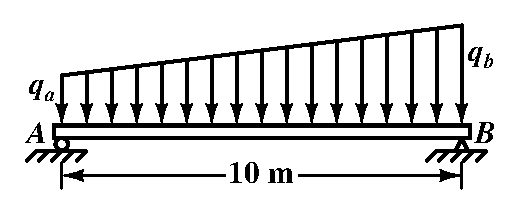
\includegraphics{src/s1s2/en/09_105/fig1}\\
    Fig. 1
    
    
  \end{center}


\item A body of weight 500N is lying on a rough plane inclined at an angle of 25$^\circ$ with
  the horizontal. It is supported by an effort (P) parallel to the plane as shown in Fig. 2. Determine
  the minimum and maximum values of P, for which the equilibrium can exist, if the angle of friction is 20$^\circ$.

  \begin{center}
  
    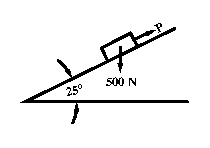
\includegraphics[scale=2]{src/s1s2/en/09_105/fig2}\\
    Fig. 2
    
    
  \end{center}



\newpage

\again

\item Determine the moment of inertia of a solid cylinder of radius R and length L about an axis passing
  through the center of gravity G and perpendicular to the axis of cylinder.

\item Two balls are projected from the same point in directions inclined at 60$^\circ$ and 30$^\circ$ to the
  horizontal. If they attain the same maximum height, find the ratio of their velocities of projection.

\item A railway wagon of weight 4 kN is moving with a velocity of 25 m/s. A force of 200N acts on the
  wagon for 2 minutes. Calculate the velocity of the wagon, if the direction of the applied force is
  (i) in the direction of motion; and (ii) in the opposite direction.

\item A rigid body rotates about a fixed axis and slows down from 300 r.p.m. to 150 r.p.m. in 2 minutes.
  Determine (i) the angular acceleration; (ii) the number of revolutions completed in 2 minutes.

\markB

\partCo

\item

  

  \iitem Determine the magnitude, direction and position of the line of action of the resultant of the
  co-planar system of forces shown in Fig. 3.

  \Or
  
\item Two smooth circular cylinders, each of weight W = 100 N and radius $r$ = 60 mm, are connected
  at their centers by a string AB of length $l$ = 160 mm and rest upon a horizontal plane,
  supporting above them a third cylinder of weight Q = 200 N and radius $r$ = 60 mm as shown in Fig. 4.
  Find the force S in the string AB and the pressures produced on the floor at the points of contact
  D and E.

  \ene


\newpage




\item 
  
  \iitem Find the forces in members BE, CE and BD for the truss shown in Fig. 5.

    \Or

  \item Calculate the moment of inertia of the section shown in Fig. 6 about the `$xx$' and `$yy$' axis
    through the centroid.

  \ene


\item


  

  \iitem A body P weighing 10 N moves vertically downwards as shown in Fig. 7 and is connected by
    a string with another body Q weighing 12 N which slides over a horizontal surface. Neglecting
    inertia of the pulley friction on its axle and extensibility of the string find the 
    acceleration of the falling weight P. The coefficient of friction between the block Q and the 
    horizontal plane is 0.4.

    \Or

  \item A bullet is fired with an initial velocity of 40m/s. from a point 20m. in front of a vertical
    wall 10m high. Find the angle of projection to enable the bullet to clear the wall.

    \ene
\newpage



\item
  \iitem A cord is wrapped around the inner core of a spool as shown in Fig.8. If the cord is pulled
  with a constant force of 300 N and if the cord wrapped around the outer core is attached to a block
  of mass 8 kg, determine the angular acceleration of the spool and the tension in the cord connected
  to block B. The spool has a mass of 25 kg and a radius of gyration with respect to the axis of rotation
  of 150 mm.

  \Or

\item A cord passes over a mass less and frictionless pulley as shown in Fig. 9, carrying a block A of
  mass 175 kg at one end and wrapped around a cylinder of mass 250 kg, which rolls on a horizontal
  plane. Determine (i) acceleration of the block A ; (ii) tension in the cord.

\ene


\ene


